\chapter{Gráficos de Resultados} \label{app:results}

Além das tabelas e gráficos exibidos no Capítulo~\ref{chap:results}, foram
gerados gráficos para \textit{tempo de espera médio por andar} para cada cenário
e estratégia simulados.

\section{Cenário \textit{Low-rise}.}

\begin{figure}[H]
  \centering
  \includegraphics[scale=0.8]{img/results/Low-rise/1_Simple_Random/averageWaitTime}
  \caption{\textit{Espera média por andar} para \textit{random} e \textit{Low-rise}.}
  \label{fig:result:low-rise:avgwt:random}
\end{figure}

\begin{figure}[H]
  \centering
  \includegraphics[scale=0.8]{img/results/Low-rise/2_Simple_NearestNeighbour/averageWaitTime}
  \caption{\textit{Espera média por andar} para \textit{nearest neighbour} e \textit{Low-rise}.}
  \label{fig:result:low-rise:avgwt:nn}
\end{figure}

\begin{figure}[H]
  \centering
  \includegraphics[scale=0.8]{img/results/Low-rise/3_Simple_BetterNearestNeighbour/averageWaitTime}
  \caption{\textit{Espera média por andar} para \textit{better nearest neighbour} e \textit{Low-rise}.}
  \label{fig:result:low-rise:avgwt:bnn}
\end{figure}

\begin{figure}[H]
  \centering
  \includegraphics[scale=0.8]{img/results/Low-rise/4_Simple_Weighted/averageWaitTime}
  \caption{\textit{Espera média por andar} para \textit{weighted} e \textit{Low-rise}.}
  \label{fig:result:low-rise:avgwt:weighted}
\end{figure}

\begin{figure}[H]
  \centering
  \includegraphics[scale=0.8]{img/results/Low-rise/5_Planning_Random/averageWaitTime}
  \caption{\textit{Espera média por andar} para \textit{planning} e \textit{Low-rise}.}
  \label{fig:result:low-rise:avgwt:planning}
\end{figure}

\section{Cenário \textit{High-rise}.}

\begin{figure}[H]
  \centering
  \includegraphics[scale=0.8]{img/results/High-rise/1_Simple_Random/averageWaitTime}
  \caption{\textit{Espera média por andar} para \textit{random} e \textit{High-rise}.}
  \label{fig:result:high-rise:avgwt:random}
\end{figure}

\begin{figure}[H]
  \centering
  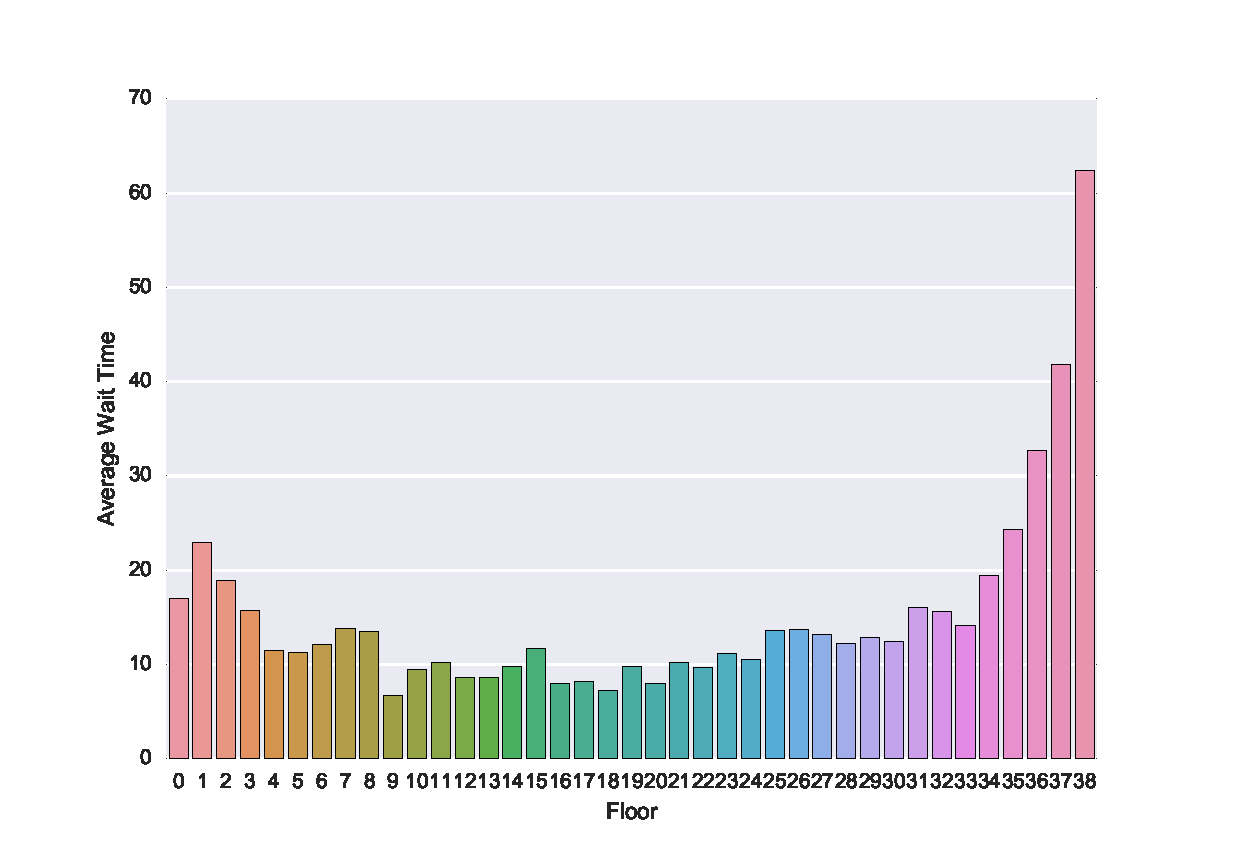
\includegraphics[scale=0.8]{img/results/High-rise/2_Simple_NearestNeighbour/averageWaitTime}
  \caption{\textit{Espera média por andar} para \textit{nearest neighbour} e \textit{High-rise}.}
  \label{fig:result:high-rise:avgwt:nn}
\end{figure}

\begin{figure}[H]
  \centering
  \includegraphics[scale=0.8]{img/results/High-rise/3_Simple_BetterNearestNeighbour/averageWaitTime}
  \caption{\textit{Espera média por andar} para \textit{better nearest neighbour} e \textit{High-rise}.}
  \label{fig:result:high-rise:avgwt:bnn}
\end{figure}

\begin{figure}[H]
  \centering
  \includegraphics[scale=0.8]{img/results/High-rise/4_Simple_Weighted/averageWaitTime}
  \caption{\textit{Espera média por andar} para \textit{weighted} e \textit{High-rise}.}
  \label{fig:result:high-rise:avgwt:weighted}
\end{figure}

\begin{figure}[H]
  \centering
  \includegraphics[scale=0.8]{img/results/High-rise/5_Planning_Random/averageWaitTime}
  \caption{\textit{Espera média por andar} para \textit{planning} e \textit{High-rise}.}
  \label{fig:result:high-rise:avgwt:planning}
\end{figure}

\section{Cenário \textit{Skyscraper}.}

\begin{figure}[H]
  \centering
  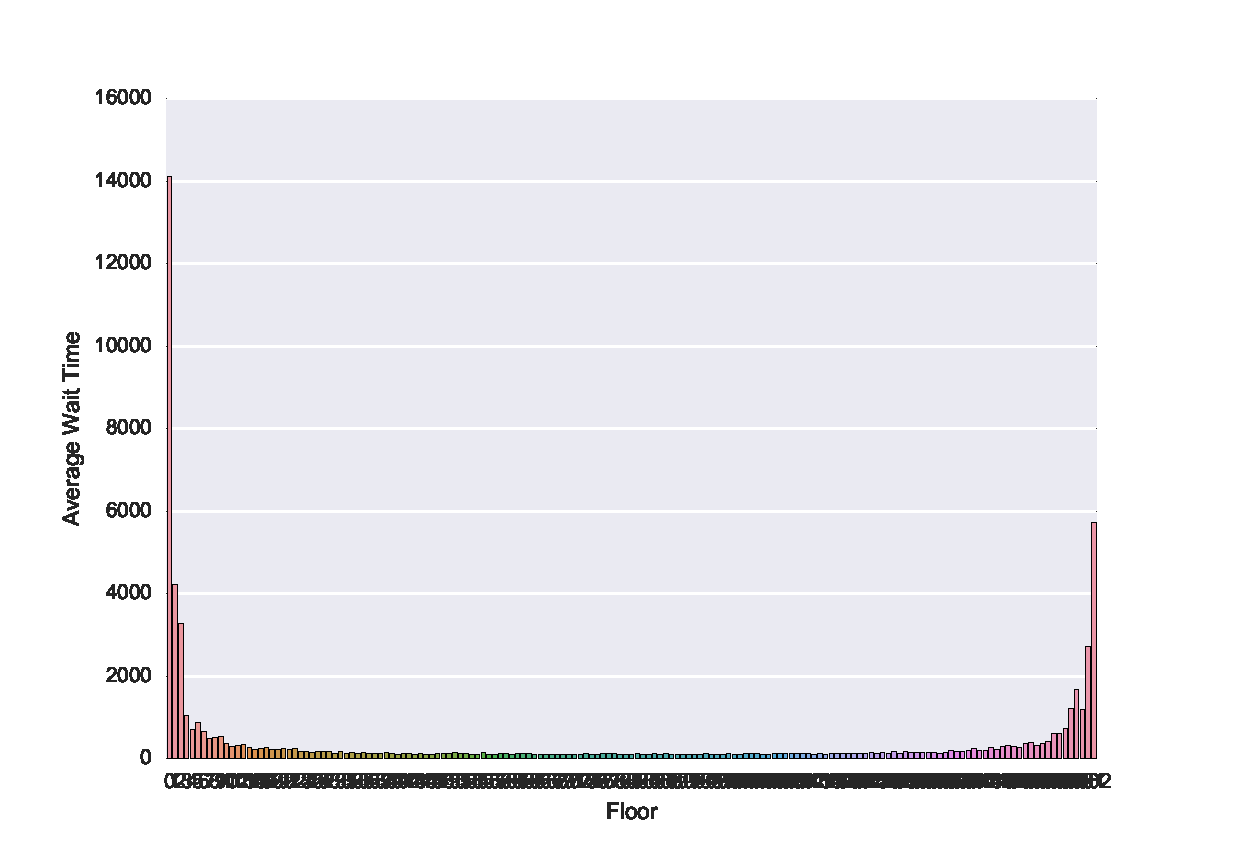
\includegraphics[scale=0.8]{img/results/Skyscraper/1_Simple_Random/averageWaitTime}
  \caption{\textit{Espera média por andar} para \textit{random} e \textit{Skyscraper}.}
  \label{fig:result:skyscraper:avgwt:random}
\end{figure}

\begin{figure}[H]
  \centering
  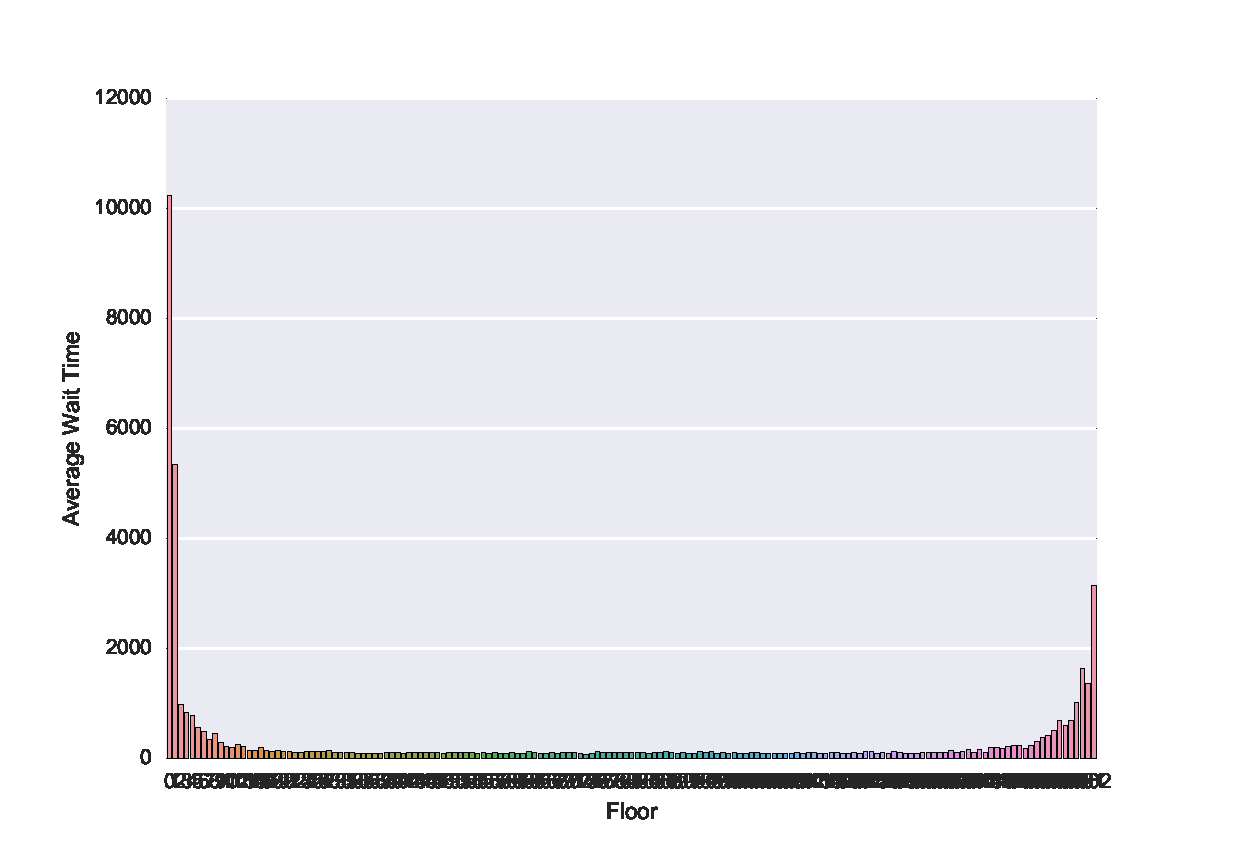
\includegraphics[scale=0.8]{img/results/Skyscraper/2_Simple_NearestNeighbour/averageWaitTime}
  \caption{\textit{Espera média por andar} para \textit{nearest neighbour} e \textit{Skyscraper}.}
  \label{fig:result:skyscraper:avgwt:nn}
\end{figure}

\begin{figure}[H]
  \centering
  \includegraphics[scale=0.8]{img/results/Skyscraper/3_Simple_BetterNearestNeighbour/averageWaitTime}
  \caption{\textit{Espera média por andar} para \textit{better nearest neighbour} e \textit{Skyscraper}.}
  \label{fig:result:skyscraper:avgwt:bnn}
\end{figure}

\begin{figure}[H]
  \centering
  \includegraphics[scale=0.8]{img/results/Skyscraper/4_Simple_Weighted/averageWaitTime}
  \caption{\textit{Espera média por andar} para \textit{weighted} e \textit{Skyscraper}.}
  \label{fig:result:skyscraper:avgwt:weighted}
\end{figure}

\begin{figure}[H]
  \centering
  \includegraphics[scale=0.8]{img/results/Skyscraper/5_Planning_Random/averageWaitTime}
  \caption{\textit{Espera média por andar} para \textit{planning} e \textit{Skyscraper}.}
  \label{fig:result:skyscraper:avgwt:planning}
\end{figure}